\section{相關研究}
本研究建構一個在Apache Spark 叢集上的Veracity真實度模型,且應用於串流XML的真實度計算,而以往的真實度研究在大部分的文獻中都是討論文件相似度。再來XML具有樹狀結構以及自描述(self-descriptive)特性,所以在分散式系統處理XML的時候,如何切割文件,但依然保有XML文件樹狀結構和父子節點的關係,以及在Hadoop或是Apache Spark的分散式架構下做XML的Query。本章節將就有關這些議題的文獻來做討論。
\subsection{XML文件特性}
XML結構與網頁使用的HTML十分相似,而兩者最大的不同為XML的設計為用來做資料傳輸,而HTML的設計是用來呈現資料。再者XML雖然可以自行定義Tag名稱,但有嚴格的巢狀結構規定。而HTML雖然在Tag的命名上沒有那麼自由,但有一些Tag沒有遵守巢狀結構的規定卻依然可以作動。\\\par
在\cite{w3sxml}\cite{2005xml}當中,針對XML的特性描述提到,XML可以表示成樹狀結構以及XML具有自描述(self-descriptive)的特性,以及XML可以使用如DTD或是Schema來規範其內容結構。\\\par
在自描述性中,XML可以使用標籤描述資料內容,如圖\ref{self}所示,文件裡面的Tag具有描述資料的功能,XML不負責呈現資料,所以程式開發者需要另外撰寫程式來完成。

\begin{figure}[H]
\centering
\graphicspath{{/Users/FUDA/Documents/masterThesis/image/}}
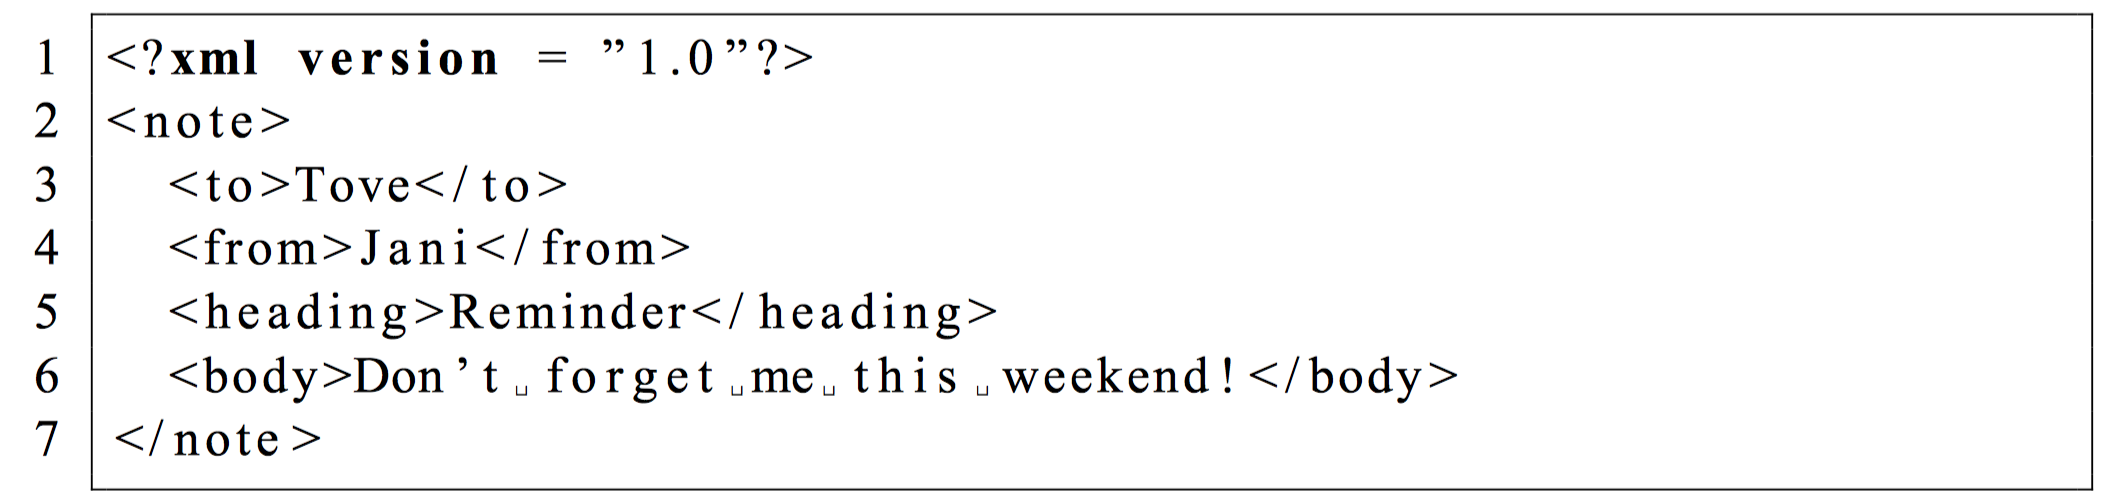
\includegraphics[scale=0.45]{xmlself.png}
\caption{XML 自描述範例}
\label{self}
\end{figure}
而XML的缺點在於需要用Tag來存放資料,以文字檔來說容量會比較大,但以現今的網路傳輸速度以及資料壓縮的技術,這也不再是問題。
\subsection{XML文件的平行化處理}
Hongjie et al.的文獻\cite{fan2018handling}提到將大型XML切割成小型的樹狀結構,存進分散式檔案系統,等到使用者的query進來之後,再將切割好的資料提取出來,使用MapReduce進行查詢。利用Hadoop的分散式系統,來到平行化query。文獻當中使用分散式檔案系統儲存XML 文件,也就是說文件在儲存之前需要經過切割。文章當中他們是採用自己設計的切割演算法,將大型XML 文件的樹狀結構切割成小型樹狀結構,接著在使用者的query進入的時候,會平行化的對這一些切割出來的小型樹狀結構作查詢。\\\par
這裡面有幾個問題點,第一點是當有多個XML文件的時候,每一份文件都會切割演算法做切割並且儲存,這時候會產生很多小文件,如何對應切割出來的小文件與原始大文件的關係,這會影響到要對哪一個文件進行處理,而文件切割和對應的部分,在\cite{eiffcientXML}當中有提到,一般在Hadoop當中,透過MapReduce切割XML文件的時候,開始標籤(<tag>)與結束標籤(</tag>)之間的關係會被切割到不同的部分,導致XML文件的節點關係不清楚,第二點是文件切割與平行化的問題,在\cite{fan2018handling}當中是使用Hadoop做處理,Hadoop 可以自行決定任務的平行化數量。而如何計算和得知切割XML的個數與平行化任務的數量各為多少是比較好的,這是在做平行化運算要面臨的問題點。\\\par

可以看到圖\ref{xmlhadoop}中紅框標示的部分即為XML文件切割完之後要進行平行化運算的部分。當中我們比較關注的是XML文件怎麼切割?被切割了幾份?以及平行畫的時候會產生的任務數量以及計算量,都是我們要考量的問題。

\begin{figure}[H]
\centering
\graphicspath{{/Users/FUDA/Documents/masterThesis/image/}}
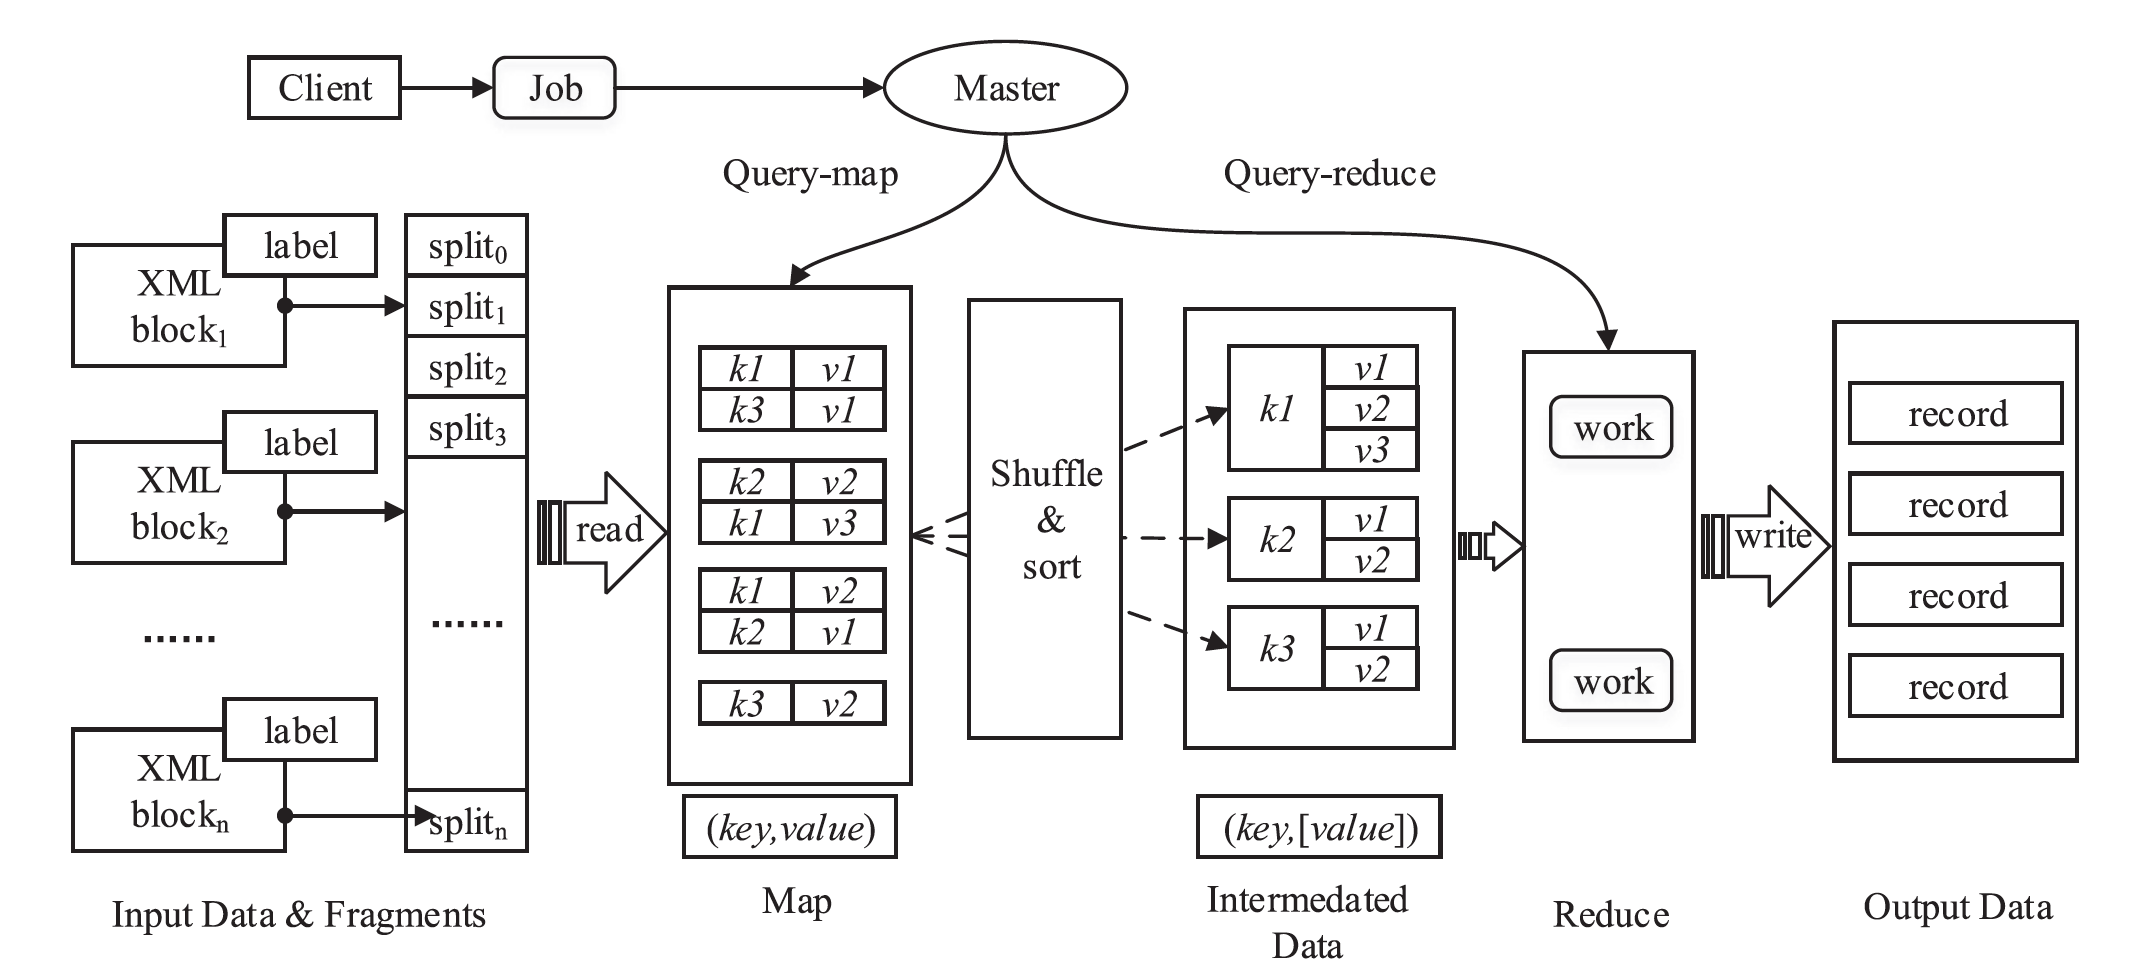
\includegraphics[scale=0.4]{xmlHadoop.png}
\caption{XML在Hadoop的切割與平行化}
\label{xmlhadoop}
\end{figure}

\subsection{XML文件相似度}
在本研究所提出的Veraicty之問題在以往的相關研究當中算少數,大部分探討是以XML文件相似度為主。在以往的研究當中會使用樹的編輯距離\cite{bille2005survey}(Edit Distance,或稱Levenshtein Distance)作相似度的比較,所謂的編輯距離為給定XML文件A與XML文件B,如果要使文件B變成跟文件A相同,需要做多少次新增、刪除以及修改的動作。在\cite{tai1979tree}當中即是採用此方法驗證兩份文件的相似度。\\\par
而在\cite{tekli2006semantic}以及\cite{tekli2012novel}當中為了增進效能,使用的是子樹(sub-tree)來做相似度的計算。而兩篇文獻不同的點在於\cite{tekli2006semantic}使用的是編輯距離,而\cite{tekli2012novel}是對於子樹的結構以及語意相似的子樹出現次數或重複次數進行計算。\cite{tekli2015approximate}則提出了基於樹編輯距離的XML語法(XML grammar)相似度驗證,並且一樣使用編輯距離來比較XML以及XML語法的相似度。\\\par
接者在\cite{algergawy2010element}當中則採用了多種的驗證方式,如Tag 名稱相似度、編輯距離、N-grams距離、Tag語意驗證等。而對於編輯距離的驗證方式除了常見的Levenshtein Distance還有使用Jaro Similarity的相似度驗證。Jaro 為兩個字串的相似度的度量,如果Jaro值越高,代表相似度越高。而另一個則為N-gram相似度,作法為將兩組欲比較之字串按照長度N切割,則可以計算兩個字串相同的子字串有多少,進而比較原字串相似度。\\\par
上述的相關研究大部分是使用編輯距離相似度演算法來做XML相似度的問題。而考量到計算效能上的問題,有幾篇的研究採用了子樹的計算來降低計算量進而強化效能。然而這樣的相似度比較對於真實度來說只是其中一個維度。而且無論是哪一種方法,在現今龐大的資料量以及串流數據的場景,皆很難完成即時性的處理。

\newpage